\documentclass[12pt, a4paper]{article}
\usepackage[utf8]{vietnam}
\usepackage{mathptmx}

% lib component
\usepackage{tikz}
\usepackage{amsmath}
\usepackage{tikz-cd}
\usepackage{amsfonts}
\usepackage{amssymb}
\usepackage{graphics}
\usepackage{array}
\usepackage{cases}
\usepackage{mdframed}
\usepackage{fancybox}
\usepackage{enumerate}
\usepackage{diagbox}
\usepackage{soul}
\usepackage{caption}
\usepackage{floatrow}
\usepackage{scrextend}
\usepackage{tikz} 
\usepackage{scrextend}
\usepackage{fancyhdr}
\usepackage{amsmath}
\usepackage[thref,thmmarks,standard,amsmath,hyperref]{ntheorem}
\usepackage{multicol}
% ----- Theorem:
%\theoremstyle{definition}
%\newtheorem{definition}{Định nghĩa}[section]

%\theoremstyle{definition}
%\newtheorem{theorem}{Định lý}[section]
%\newtheorem*{remark}{Nhận xét}
%\newtheorem{vd}{Ví dụ}[section]
%\newtheorem{bt}{Bài tập}[section]
%\newtheorem{tc}{Tính chất}[section]
%\newtheorem{md}{Mệnh đề}[section]
%\newtheorem{cy}{Chú ý}[section]
%\newtheorem{nx}{Nhận xét}[section]

% ----- Constant:
% Thông tin về đồ án
\def\author{Nguyễn Bùi Nam Trường}
\def\mssv{20185418}
\def\SCHOOL{TRƯỜNG ĐẠI HỌC BÁCH KHOA HÀ NỘI}
\def\school{Trường Đại học Bách Khoa Hà Nội}
\def\INSTITUTE{VIỆN TOÁN ỨNG DỤNG VÀ TIN HỌC}
\def\institute{Viện Toán ứng dụng và Tin học}


\def\instructor{Nguyễn Huy Trường}
\def\INSTRUCTOR{TS. Nguyễn Huy Trường}

\def\PROJECT{LẬP TRÌNH ANDROID}
\def\project{Lập trình Android}
\def\projects{Lập trình Android với React Native}

% ----- Style:
\usepackage{xcolor}
\usepackage[left=3.5cm, right=2cm, top=3.5cm, bottom=3cm]{geometry}
\usepackage[colorlinks=true, allcolors=black, unicode]{hyperref}
\changefontsizes[18pt]{13pt}
\setlength{\parindent}{0.6cm}
\usepackage{indentfirst}
\setlength{\parskip}{2pt}
\renewcommand{\baselinestretch}{1.4}
\setlength{\baselineskip}{18truept}
\renewcommand{\headrulewidth}{0.5pt}
\renewcommand{\footrulewidth}{0.5pt}
\usepackage[]{hyperref}

% ----- Format:
\pagestyle{fancy}
\fancyhf{}
\usepackage{enumerate}
\usepackage{enumitem}
\lhead{\normalsize \projects}
\rhead{\normalsize \project}
\lfoot{\normalsize \author - \mssv}
\rfoot{Trang \thepage}
% \renewcommand\thesection{Chương \Roman{section}}
% \renewcommand\thesubsection{\arabic{subsection}}

% ----- Mục lục:
\newcommand{\nocontentsline}[3]{}
\newcommand{\tocless}[2]{\bgroup\let\addcontentsline=\nocontentsline#1{#2}\egroup}

% ------------------------------------------------------- %

\begin{document}
    	% ----- Trang bìa:
        \begin{titlepage}
	\begin{tikzpicture}[remember picture,overlay,inner sep=0,outer sep=0]
		\draw[blue!70!black,line width=5pt] 
		([xshift=-2cm,yshift=-2cm]current page.north east) coordinate (A)--
		([xshift=2cm,yshift=-2cm]current page.north west) coordinate(B)--
		([xshift=2cm,yshift=2cm]current page.south west) coordinate (C)--
		([xshift=-2cm,yshift=2cm]current page.south east) coordinate(D)--cycle;
		
		\draw ([yshift=0.5cm,xshift=-0.5cm]A)-- ([yshift=0.5cm,xshift=0.5cm]B)-- ([yshift=-0.5cm,xshift=0.5cm]B) --([yshift=-0.5cm,xshift=-0.5cm]B)--([yshift=0.5cm,xshift=-0.5cm]C)--([yshift=0.5cm,xshift=0.5cm]C)--([yshift=-0.5cm,xshift=0.5cm]C)-- ([yshift=-0.5cm,xshift=-0.5cm]D)--([yshift=0.5cm,xshift=-0.5cm]D)--([yshift=0.5cm,xshift=0.5cm]D)--([yshift=-0.5cm,xshift=0.5cm]A)--([yshift=-0.5cm,xshift=-0.5cm]A)--([yshift=0.5cm,xshift=-0.5cm]A);
		
		
		\draw ([yshift=-0.3cm,xshift=0.3cm]A)-- ([yshift=-0.3cm,xshift=-0.3cm]B)--
		([yshift=0.3cm,xshift=-0.3cm]B) --([yshift=0.3cm,xshift=0.3cm]B)--([yshift=-0.3cm,xshift=0.3cm]C)--([yshift=-0.3cm,xshift=-0.3cm]C)--([yshift=0.3cm,xshift=-0.3cm]C)-- ([yshift=0.3cm,xshift=0.3cm]D)--([yshift=-0.3cm,xshift=0.3cm]D)--([yshift=-0.3cm,xshift=-0.3cm]D)--([yshift=0.3cm,xshift=-0.3cm]A)--([yshift=0.3cm,xshift=0.3cm]A)--([yshift=-0.3cm,xshift=0.3cm]A);
	\end{tikzpicture}
	\begin{center}
		\begin{large}
			\textbf{\SCHOOL}\\
			\textbf{\INSTITUTE}\\
		\end{large}
		\centerline{--------------------o0o--------------------}
		\vspace{0.5cm}
		
\includegraphics[scale=0.6]{images/logo.jpg}\\
		\vspace{0.5cm}
		{\fontsize{28pt}{1}\selectfont \textbf{\PROJECT}}\\
		\vspace{0.5cm}
		{\fontsize{16pt}{1}\selectfont \textbf{ĐỒ ÁN II}}\\
		{\fontsize{13pt}{1}\selectfont \textbf{Chuyên ngành: TOÁN TIN}}\\
		{\fontsize{13pt}{1}\selectfont \textbf{\textcolor{red}{Chuyên sâu: \projects}}}
	\end{center}
	\vspace{0.5cm}
	\begin{center}
		\begin{tabular}{ll}
			Giảng viên hướng dẫn & : \textbf{\INSTRUCTOR}\\
			Nhóm sinh viên thực hiện & : \textbf{\author}\\
			MSSV & : \textbf{20185418}\\
		\end{tabular}
	\end{center}
	\vspace{0.5cm}
	\begin{center}
		{\bf HÀ NỘI, tháng ../2022}
	\end{center}
\end{titlepage}
	
        % ----- Nhận xét của Giáo viên
        % \newpage
\section*{\centering Lời nói đầu}
\addcontentsline{toc}{section}{Lời nói đầu}
% Giới thiệu về lập trình android

% Giới thiệu về React Native

% Chọn đề tài

% Tóm tắt nội dung đồ án

% Lời cảm ơn

\begin{flushright}
	\begin{tabular}{rc}
		& Hà Nội, ngày .. tháng .. năm 2022 \\
		& Sinh viên thực hiện \\	
		\\
		& Nguyễn Bùi Nam Trường \\
	\end{tabular}
\end{flushright}
\newpage
        
        % ----- Lời nói đầu:
        % \newpage
\section*{\centering Lời nói đầu}
\addcontentsline{toc}{section}{Lời nói đầu}
% Giới thiệu về lập trình android

% Giới thiệu về React Native

% Chọn đề tài

% Tóm tắt nội dung đồ án

% Lời cảm ơn

\begin{flushright}
	\begin{tabular}{rc}
		& Hà Nội, ngày .. tháng .. năm 2022 \\
		& Sinh viên thực hiện \\	
		\\
		& Nguyễn Bùi Nam Trường \\
	\end{tabular}
\end{flushright}
\newpage
        
        % ----- Mục lục:
        \tableofcontents	
        
        % ----- Kí hiệu và từ viết tắt:
        % \newpage
\section*{\centering Lời nói đầu}
\addcontentsline{toc}{section}{Lời nói đầu}
% Giới thiệu về lập trình android

% Giới thiệu về React Native

% Chọn đề tài

% Tóm tắt nội dung đồ án

% Lời cảm ơn

\begin{flushright}
	\begin{tabular}{rc}
		& Hà Nội, ngày .. tháng .. năm 2022 \\
		& Sinh viên thực hiện \\	
		\\
		& Nguyễn Bùi Nam Trường \\
	\end{tabular}
\end{flushright}
\newpage
    
        % ----- Nội dung chính
        % % Chương 1: Giới thiệu về Android
%     1.1 Khái niệm về Android
%     1.2 Kiến trúc của Android
% Chương 2: Môi trường lập trình Android
% Chương 3: Giới thiệu về React và ReactNative


\newpage
% ----- Chương 1:
\section{Giới thiệu về Android}

\subsection{Khái niệm về Android}
Trước hết, Hệ điều hành (Operating System - OS) là phần mềm hệ thống quản lý phần cứng máy tính, phần mềm và cung cấp các dịch vụ chung cho các chương trình máy tính.
Android là hệ điều hành dựa trên mã nguồn mở Linux OS cho các thiết bị di động và các thiết bị thông minh như máy tính bảng, laptop, netbook, smartbook, TV thông minh(Google TV),\dots Hiện nay, một số hệ điều hành cho thiết bị di động: Android, OS X (iPhone), Windows Mobile, Symbian,\dots Tuy nhiên, hệ điều hành được sử dụng nhiều nhất là Android và OS X.

% Điểm nổi bật của Android
Ngay từ khi ra mắt, Android đã gây ấn tượng mạnh khi đây là đứa con của Goodle sử dụng giấy phép mã nguồn mở. Android là sản phẩm kết tinh từ ý tưởng của Khối Liên minh thiết bị cầm tay mở do Google dẫn đầu, gồm 34 thành viên với các công ty hàng đầu về công nghệ và di động toàn cầu như Qualcomm, Intel, Motorola, Texas Instruments và LG Electronics, các nhà mạng như T-Mobile, Sprint Nextel, NTT DoCoMo và China Mobile.

% Đặc tính mở của Android
Với đặc tính "mở", Android cho phép các nhà phát triển có thể sử dụng miễn phí bộ Kit Android Software Development để xây dựng các ứng dụng của mình. Ví dụ, một ứng dụng có thể gọi bất kì chức năng lõi của điện thoại như thực hiện gọi, gửi tin nhắn, sử dụng máy ảnh,\dots Điều này thực sự thu hút các nhà phát triển sáng tạo ra các phần mềm hấp dẫn, từ đó tạo ra một cộng đồng phát triển lớn - là nguyên nhân đến sự phổ biến của Android như hiện nay.

\subsection{Kiến trúc của Android}
Để bắt đầu lập trình với Android, chúng ta cần nghiên cứu qua bản thân HĐH Android, chúng ta không cần hiểu quá chi tiết, nhưng trước hết là cần có cái nhìn chung và toàn diện nhất về Android.

Android Platform bao gồm đầy đủ các tính năng HĐH Android, các ứng dụng và các tâng trung gian để nhà phá triển có thể mở rộng, tùy chỉnh thêm theo nhu cầu của họ. Có 4 tầng cơ bản trong HĐH Android: Linux Kernel, Native Libraries, Android Runtime, Application Framework,\dots Các tầng làm việc có sự liên kết với nhau.
\begin{enumerate}
    \item{\textit{Tầng Linux Kernel:}}
    Đây là tầng nhân của HĐH Android, Linux Kernel giúp hệ điều hành có thể giao tiếp với phần cứng của thiết bị như: camera,  USB, Wifi, Bluetooth, Display, Power Management,\dots  Linux Kernel chịu trách nhiệm cho các trình điều khiển thiết bị, quản lý nguồn điện, quản lý bộ nhớ, quản lý thiết bị và truy cập tài nguyên. Kernel hoạt động như một lớp trừu tượng giữa phần cứng và phần mềm còn lại của hệ thống.
    \item{\textit{Native Libraries:}}
    Native Libraries là tập hợp của nhiều thư viện như WebKit, OpenGL, FreeType, SQLite, Media, SSL,\dots 
    \item{\textit{Tầng Android Runtime:}}
    Android Runtime cung cấp một thành phần quan trọng được gọi là DVM (Dalvik Virtual Machine - máy ảo) có trách nhiệm chạy ứng dụng android.
    DVM thực thi các file có định dạng .dex (Dalvik Excutable), định dạng này là định dạng được tối ưu hóa về bộ nhớ.
    \newline
    DVM có phần tương tự như JVM (Java Virtual Machine) nhưng được tối ưu hóa cho các thiết bị di động như tiêu thụ ít bộ nhớ hơn và tăng hiệu suất hoạt động tốt hơn.
    \item{\textit{Tầng Application Framework:}}
    Application Framework bao gồm tập hợp những API cho phép các nhà phát triển ứng dụng được phép sử dụng các dịch vụ này trong các ứng dụng của họ.
\end{enumerate}
Ở góc độ người dùng, ta có thêm tầng Application - là các ứng dụng do nhà phát triển ứng dụng viết. Dưới đây là sơ đồ tương quan liên kết giữa các tầng:
\newline
\begin{figure}[!ht]
    \centering
    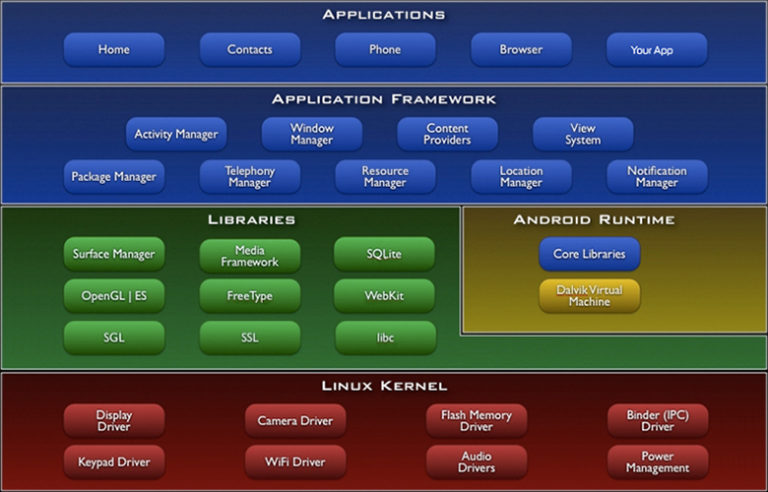
\includegraphics[scale=0.5]{images/android-flatform.jpg}
    \caption{Sơ đồ tương quan liên kết giữa các tầng}
\end{figure}



% ----- Chương 2:
\section{Giới thiệu về React Native}

\subsection{Giới thiệu}
React Native là một Framework, do công ty Công nghệ Meta (trước đây là Facebook) phát triển, nhằm giải quyết vấn đề về hiệu năng và việc phải sử dụng nhiều ngôn ngữ native trên nền tảng di động.
\newline
React Native cho phép xây dựng và phát triển ứng dụng native đa nền tảng một cách dễ dàng, khác với HTML5 App, Mobile Web App, Hybrid App. Mục đích khi tạo ra React Native là khắc phục các điểm yếu của ứng dụng web, giúp cho nhà lập trình tiết kiệm thời gian, công sức bởi sự hỗ trợ đắc lực từ JavaScript.
\newline
React Native là một trong những framework sử dụng cấu hình thiết kế tương tự như React. Có thể nói, biết về React là biết được 80\% về React Native. Tuy nhiên, đồ án này sẽ trình bày đủ các thông tin cả về React.

\subsection{Lịch sử phát triển}
Năm 2012 Mark Zuckerberg đã phát biểu: "Sai lầm lớn nhất của chúng tôi khi làm công ty là dựa trên quá nhiều HTML hơn là môi trường phát triển gốc". Ông hứa rằng Facebook sẽ sớm cung cấp trải nghiệm di động tốt hơn.
\newline
Kỹ sư Jordan Walke tại Facebook đã tìm ra cách xây dựng các thành phần UI cho iOS bằng một luồng JavaScript. Họ quyết định tổ chức cuộc thi Hackathon để hoàn thiện nguyên mẫu hệ thống để có thể xây dựng các ứng dụng di động gốc (native app) bằng công nghệ này.
\newline
Sau nhiều tháng phát triển, Facebook đã phát hành phiên bản đầu tiên cho React Native vào năm 2015. Trong một cuộc hội thảo công nghệ, Christopher Chedeau cho biết Facebook đã sử dụng React Native trong phát triển ứng dụng nhóm và ứng dụng quản lí quảng cáo của họ.
\newline
Với cộng đồng phát triển ứng dụng lớn, ngày nay React Native trở thành framework được ưa chuông trong việc xây dựng ứng dụng native.

\subsection{Lý do React Native được ưa chuộng}
Để biết tại sao React Native lại được ưa chuộng, ta đề cập đến các ứng dụng phổ biến trước đây là Hybrid Apps. Hybrid App được hiểu là ứng dụng được xây dựng dựa trên các công nghệ web phổ biến là CSS, Javascript, HTML. Như vậy, ứng dụng được xây dựng lớn, cần phát triển lâu dài thì sẽ không đảm bảo được hiệu năng.
% Trong khi đó, Native App có thể nâng cao tương tác nhanh hơn do chúng được xây dựng với framework có nguồn gốc phát triển từ platform. Từ đó, Native App có khả năng hoạt động ở chế độ ngoại tuyến, có thể tiếp cận cả với những khách hàng không có internet.
\newline
Trong khi đó, React Native lại có những ưu điểm sau:
\begin{enumerate}
    \item {Tiết kiệm thời gian học:} Việc học từng loại ngôn ngữ cho từng nền tảng thường rất khó và mất nhiều thời gian. Tuy nhiên với React Native, lập trình viên chỉ cần học duy nhất một bộ công cụ.
    \item {Tái sử dụng code:} Trong lập trình phần mềm, React Native là công cụ tái sử dụng code hiệu quả nhất mang lại các lợi thế như duy trì ít code, tận dụng tốt nguồn nhân lực,\dots
    \item {Hot reloading:} Khi phát triển ứng dụng, nhà phát triển không tốn quá nhiều thời gian để tổng hợp app mỗi khi có sự thay đổi mà chỉ cần làm mới app trong thiết bị hoặc giả lập
\end{enumerate}
Chính vì lý do trên mà hiện nay, React Native  đang dần trở thành lựa chọn số một cho công việc xây dựng app của hầu hết các công ty lớn. Cũng từ việc được ưa chuộng khiến cho cộng đồng phát triển lớn, từ đó tạo thành vòng lặp khiến các nhà phát triển mới tiếp cận đều chon React Native.

\subsection{Nguyên lý hoạt động}
Về cơ bản, React Native hoạt động bằng cách tích hợp cho ứng dụng đi động 2 thread là JS thread và Main thread.
\begin{enumerate}
    \item{\textit{Main thread}}: giữ vai trò cập nhật giao diện người dùng UI và xử lý các tương tác của người dùng ngay sau đó.
    \item{\textit{JS thread}}: thực thi và xử lý các code JavaScript.
\end{enumerate}
Hai thread này hoạt động độc lập với nhau và giao tiếp qua một cầu nối trung gian.

\subsection{Một số ứng dụng sử dụng react native}
Với việc được ưa chuộng và có cộng đồng phát triển lớn, thế giới càng ngày càng có nhiều ứng dụng sử dụng React Native ra đời. Một số ứng dụng có thể kế đến như sau:
\begin{enumerate}
    \item {\textit{Facebook:}} là công ty phát triển React Native, sau khi phát triển xong framework này, Meta đã chuyển đổi tính năng Event Dashboard cho iOS sang React Native để kiểm tra hiệu suất ứng dụng, từ đó cắt giảm thời gian tìm hiểu thị trường đi một nửa
    \item {\textit{Facebook Ads:}} Đến thời điểm hiện tại, tất cả ứng dụng quảng cáo trên Facebook đều được sử dụng React Native.
    \item {\textit{Instagram:}} Sau khi được Meta mua lại, ứng dụng này cũng được chuyển đổi sử dụng React Native, cụ thể chế độ Push Notifications đã được triển khai dưới dạng WebView và không yêu cầu xây dựng cơ sở hạ tầng Navigation vì UI khá đơn giản.
\end{enumerate}
        
        % ----- Kết luận
        % \newpage
\section*{\centering Kết luận}
\addcontentsline{toc}{section}{Kết luận}
Sau quá trình nghiên cứu và tìm hiểu về chủ đề \projects, em đã có thêm kiến thức nhất định về lập trình Android nói riêng và ứng dụng Native nói chung, cùng với đó là những kĩ năng, kinh nghiệm trong việc xây dựng và phát triển phần mềm.

Mặc dù đã rất cố gắng trong việc nghiên cứu và thực hiện đô án, nhưng do thời gian hạn cũng như sự hiểu biết của bản thân em còn hạn chế nên đồ án chỉ dừng lại ở việc tìm hiểu về Android, React Native mà chưa đi sâu vào phát triển ứng dụng hoàn chỉnh, giải quyết bài toàn thực trong cuộc sống. Bài đồ án này cũng giúp em mở ra định hướng nghiên cứu thêm cách phát triển ứng dụng React Native lớn với quy mô nhóm: code convention, design partent đối với React Native,\dots Nếu có cơ hội, em sẽ tìm hiểu và trình bày ở đồ án sau.

\textit{Em xin chân thành cảm ơn!}
\newpage
        
        % ----- Tài liệu tham khảo
        % \newpage
\section*{\centering Tài liệu tham khảo}
\addcontentsline{toc}{section}{Tài liệu tham khảo}

\textbf{Tài liệu do nhà phát hành cung cấp}
\begin{enumerate}
	\item \url{https://reactnative.dev/docs}.
	\item \url{https://reactjs.org/docs}.
\end{enumerate}

\textbf{Tài liệu từ các thông tin tổng hợp trên trình duyệt}
\begin{enumerate}
	\item \url{https://teamvietdev.com/thanh-phan-kien-truc-android/}.
	\item \url{https://wikipedia.org/wiki/React_Native}.
	\item \url{https://vietnix.vn/nodejs-la-gi/}.
	\item \url{https://vietnix.vn/nodejs-la-gi/}.
\end{enumerate}
\newpage
\end{document}